\documentclass[a4paper,12 pt]{article}
\usepackage[T2A]{fontenc}
\usepackage[utf8]{inputenc}
\usepackage[english, russian]{babel}
\usepackage{geometry}
\usepackage{float}
\usepackage{amsfonts}
\usepackage{array}
\newcolumntype{C}[1]{>{\centering\arraybackslash}p{#1}}
 \geometry{
 a4paper,
 top=25mm,
 }
\usepackage{amsmath, amsfonts, amssymb, amsthm, mathtools, indentfirst, float, wrapfig}
\usepackage{wrapfig}
\usepackage{graphicx}
\graphicspath{{pictures/}}
\DeclareGraphicsExtensions{.pdf,.png,.jpg}
\begin{document}
    \begin{titlepage}
    \begin{center}
        \vspace{4cm}
        \huge {\textbf{Отчет о выполнении лабораторной работы 3.7.3 }}
        {} \\
        \vspace{1cm}
        \Large {\textbf{Длинная линия}} \\
        \Large {\textbf{}} \\
        \vspace{10cm}
        \begin{flushright}
        \begin{minipage}{.45\textwidth}
        \normalsize{\textbf{Студент:} Копытова Виктория Сергеевна}\\
        \textbf{Группа:} Б03-304\\
        \end{minipage}
        \end{flushright}   
    \end{center}
    \end{titlepage}
\newpage
 
\section{Аннотация}
\textbf{Цель работы:} ознакомится и проверить на практике теорию распространения
электрических сигналов вдоль длинной линии; измерить амплитудо- и фазово-частотные
характеристики коаксиальной линии; определить погонные характеристики такой
линии; на примере модели длинной линии изучить вопрос распределения амплитуды
колебаний сигнала по длине линии.

\textbf{В работе используются:} осциллограф АКТАКОМ ADS-6142H; генератора АКИП 3420/1; бухта с
коаксиальным кабелем pk 50-4-11; схематический блок "модель длинной линии"; магазин
сопротивления Р33, соединительные провода.
	

\section{Теоретические сведения}

\begin{figure}
    \centering
    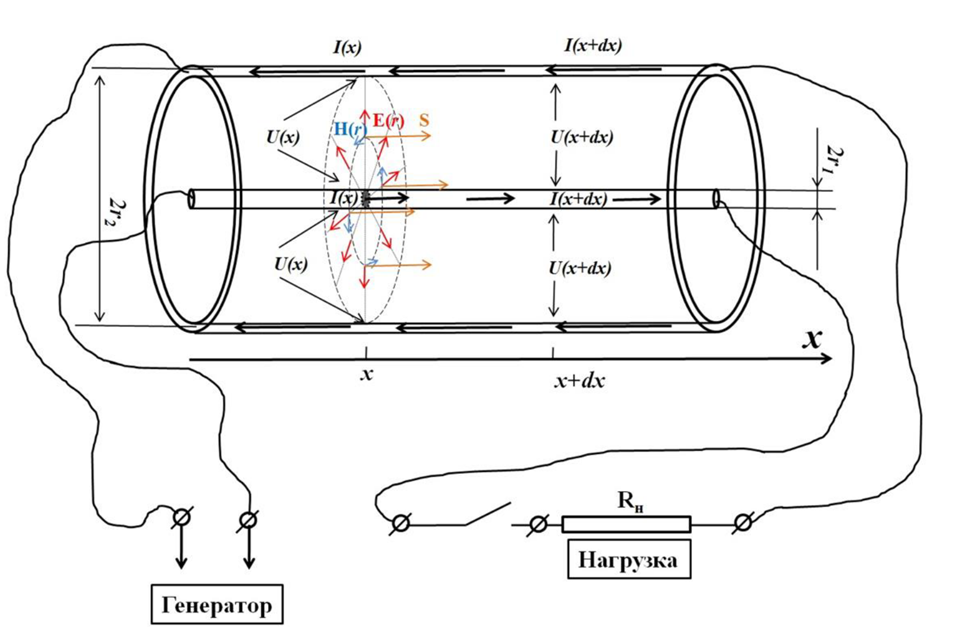
\includegraphics[scale = 0.7]{1.png}
    \caption{Схематическое изображение элемента dx длинного коаксиального кабеля}
    \label{fig:enter-label}
\end{figure}

Рассмотрим элемент dx длинного коаксиального кабеля. Этот элемент представляет
собой изолированный коаксиальный проводящий (медный) цилиндр некоторого радиуса $r_2$, на оси которого расположен сплошной тонкий проводник (медный) круглого сечения с 

радиусом $r_{1}$. Пространство между этими проводниками заполнена средой, обладающей диэлектрической проницаемостью $\varepsilon$ и магнитной восприимчивостью $\mu$. Как известно, такой элемент обладает индуктивностью


\begin{equation*}
d L=2 \mu \ln \left(r_{2} / r_{1}\right) d x \tag{1}
\end{equation*}


Удельная (погонная) индуктивность единицы длины такого кабеля:


\begin{equation*}
L_{x}=\frac{d L}{d x}=2 \mu \ln \left(r_{2} / r_{1}\right) \tag{2}
\end{equation*}


Два проводника, образующих этот элемент $d x$ коаксиального кабеля, должны обладать взаимной ёмкостью. Можно показать, что ёмкость элемента $d x$ коаксиального кабеля определяется выражением:


\begin{equation*}
d C=\frac{\varepsilon}{2 \ln \left(r_{2} / r_{1}\right)} d x \tag{3}
\end{equation*}


а его удельная (погонная) ёмкость единицы длины равна:


\begin{equation*}
C_{x}=\frac{d C}{d x}=\frac{\varepsilon}{2 \ln \left(r_{2} / r_{1}\right)} . \tag{4}
\end{equation*}


Когда по такому кабелю передаётся сигнал, в его центральной жиле и внешней оболочке возникают взаимно противоположные токи $I(x)$, а также электрическое напряжение $U(x)$ между внешним и внутренним проводниками. При высоких частотах $v$ сигналов, распространяющихся в кабеле (когда длина кабеля $l>V / v$, где $V$ - характерная скорость распространения сигнала в кабеле, эта скорость, как правило, порядка скорости света) $I(x)$ и $U(x)$ вообще говоря зависят от координаты $x$.

Изменение напряжения на концах элемента $d x$ вызваны возникновением ЭДС индукции и падением напряжения в результате омического сопротивления проводников:


\begin{equation*}
U(x+d x)-U(x)=-\frac{L_{x} d x}{c^{2}} \frac{\partial I}{\partial t}-R_{x} d x I, \tag{5}
\end{equation*}


где погонное сопротивление


\begin{equation*}
R_{x}=\frac{d R}{d x}=\frac{1}{\sigma \cdot S} \tag{6}
\end{equation*}


здесь $\sigma$ - удельная проводимость материала проводников, $S$ - площадь их поперечного сечения.

Изменение силы тока вызвано тем, что некоторая часть электрического заряда $q$ как бы "перетекает на "обкладки" конденсатора, роль которых играют проводники коаксиального кабеля:


\begin{equation*}
I(x+d x)-I(x)=-\frac{\partial q}{\partial t} \tag{7}
\end{equation*}


где $q=C_{x} d x U$.\\
Представим уравнения (5) и (7) в виде системы, описывающей распространение сигнала вдоль длинной линии:

\[
\left\{\begin{array}{l}
U(x)=U(x+d x)+\frac{L_{x} d x}{c^{2}} \frac{\partial I}{\partial t}+R_{x} d x I,  \tag{8}\\
I(x)=I(x+d x)+\frac{\partial q}{\partial t} .
\end{array}\right.
\]

Эту систему уравнений называют телеграфными уравнениями. Разделим оба уравнения на длину элемента $d x$ и, воспользовавшись определением дифференциалов, перепишем (8) следующим образом:

\[
\left\{\begin{array}{l}
\frac{\partial I}{\partial x}=-C_{x} \frac{\partial U}{\partial t}  \tag{9}\\
\frac{\partial U}{\partial x}=-\frac{L_{x}}{c^{2}} \frac{\partial I}{\partial t}-R_{x} I
\end{array}\right.
\]

Из (9) выразим перекрёстные производные:

\[
\left\{\begin{array}{l}
\frac{\partial^{2} I}{\partial x \partial t}=-C_{x} \frac{\partial^{2} U}{\partial^{2} t}  \tag{10}\\
\frac{\partial^{2} U}{\partial x^{2}}=-\frac{L_{x}}{c^{2}} \frac{\partial^{2} I}{\partial x \partial t}-R_{x} \frac{\partial I}{\partial x}
\end{array}\right.
\]

Из (9) и (10) получаем волновое уравнение для напряжения $U(x)$


\begin{equation*}
\frac{\partial^{2} U}{\partial x^{2}}=\frac{L_{x} C_{x}}{c^{2}} \frac{\partial^{2} U}{\partial t^{2}}+R_{x} C_{x} \frac{\partial U}{\partial t} . \tag{11}
\end{equation*}


Или в каноническом виде:


\begin{equation*}
\frac{\partial^{2} U}{\partial t^{2}}-V_{\phi}^{2} \frac{\partial^{2} U}{\partial x^{2}}+\gamma \frac{\partial U}{\partial t}=0 \tag{12}
\end{equation*}


где введены следующие обозначения для фазовой скорости:


\begin{equation*}
V_{\phi}=\frac{c}{\sqrt{L_{x} C_{x}}} \tag{13}
\end{equation*}


и декремента затухания:


\begin{equation*}
\gamma=R_{x} C_{x} V_{\phi}^{2} . \tag{14}
\end{equation*}


Подставляя (2) и (4) в выражение для фазовой скорости (13), легко видеть, что, эта скорость имеет тот же вид, как и скорость распространения обычных электромагнитных волн в некоторой среде с диэлектрической проницаемостью $\varepsilon$ и магнитной восприимчивостью $\mu$ :


\begin{equation*}
V_{\phi}=\frac{C}{\sqrt{\varepsilon \mu}} . \tag{15}
\end{equation*}


Решение (12) удобно искать в виде:


\begin{equation*}
U(x, t)=U_{0} e^{-i \omega t} e^{(-\alpha+i k) x} \tag{16}
\end{equation*}


Из первого уравнения системы (9) легко установить характер изменения силы тока в длинной линии:


\begin{equation*}
I(x, t)=U_{0} \frac{C_{x} \omega}{k+i \alpha} e^{-i \omega t} e^{(-\alpha+i k) x} \tag{17}
\end{equation*}


Из (16) и (17) видно, что отношение силы тока и напряжения в длинной линии не зависят от времени и координаты. Это отношение называют волновым сопротивлением (импедансом):


\begin{equation*}
Z(\omega, k)=\frac{U(x, t)}{I(x, t)}=\frac{k+i \alpha}{C_{x} \omega} . \tag{18}
\end{equation*}


В пределе малых затуханий $\alpha<<\omega$


\begin{equation*}
Z(\omega, k) \approx \frac{k}{C_{x} \omega}=\frac{1}{C_{x} V_{\phi}}=\frac{1}{c} \sqrt{\frac{L_{x}}{C_{x}}} \tag{19}
\end{equation*}


Если в конце такую длинную линию замкнуть на сопротивление


\begin{equation*}
R_{0}=\frac{1}{c} \sqrt{\frac{L_{x}}{C_{x}}} \tag{20}
\end{equation*}


то бегущая вдоль длинной линии волна "будет воспринимать" нагрузку как бесконечное продолжение этой длинной линии. Другими словами, когда длинная линия подключена к нагрузке с сопротивлением $R_{0}$, отражённой волны не возникает. Во всех остальных случаях, когда $R \neq R_{0}$ (в том числе и в частных случаях незамкнутого конца, когда $R \rightarrow \infty$ и короткозамкнутой линии, когда $R=0$ ) возникает отражённая волна, описываемая выражением (сравни с (13)):\\
$U(x, t)=U_{0} e^{-i \omega t} e^{-(\alpha+i k) x}$, которое также удовлетворяет решению системы (9).

Подставляя (16) в (12) получаем характеристическое уравнение:


\begin{equation*}
-\omega^{2}-V_{\phi}^{2}(-\alpha+i k)^{2}-i \omega \gamma=0 \tag{21}
\end{equation*}


Или, разделяя действительную и мнимую части, приходим к системе:

\[
\left\{\begin{array}{l}
\omega^{2}=V_{\phi}^{2}\left(k^{2}-\alpha^{2}\right)  \tag{22}\\
2 \alpha k V_{\phi}^{2}=\omega \gamma
\end{array}\right.
\]

Из (22) следует (в пределе малых затуханий $\alpha<<\omega$ ):


\begin{align*}
\alpha=\frac{\omega}{V_{\phi}} \sqrt{\frac{\sqrt{1+(\gamma / \omega)^{2}}-1}{2}} & \approx \frac{\omega}{V_{\phi}} \sqrt{\frac{\gamma^{2}}{4 \omega^{2}}}=\frac{\gamma}{2 V_{\phi}}=R_{\chi} C_{x} \frac{V_{\phi}}{2},  \tag{23}\\
k & =\frac{\omega}{V_{\phi}} . \tag{24}
\end{align*}


Таким образом, амплитуда напряжения на нагрузке (в конце длинной линии) будет иметь вид:


\begin{equation*}
U_{n}(t)=U_{0} e^{-\alpha l} e^{i k l} e^{-i \omega t} . \tag{25}
\end{equation*}


При этом амплитуда колебаний на согласованной нагрузке (в конце длинной линии) имеет вид:


\begin{equation*}
U_{n}=U_{0} e^{-\alpha l}, \tag{26}
\end{equation*}


и набег фазы сигнала на выходе (в конце длинной линии) относительно входного сигнала (вначале длинной линии) будет иметь вид:


\begin{equation*}
\Delta \varphi=k l . \tag{27}
\end{equation*}


Так как модуль волнового вектора $k$ прямо пропорционален частоте сигнала $\omega$ (см. выражение (24)) следует понимать, что разность фазы $\Delta \varphi$ монотонно увеличивается с увеличением $\omega$.

Из (26) и (27) легко экспериментально определить декремент затухания $\alpha$ и волновое число $k$ для различных $\omega$ :


\begin{gather*}
\alpha(\omega)=\frac{1}{l} \ln \left(\frac{U_{0}}{U_{H}}\right),  \tag{28}\\
k(\omega)=\frac{\Delta \varphi}{l} \tag{29}
\end{gather*}



\section{Ход работы}
\begin{figure}[H]
    \centering
    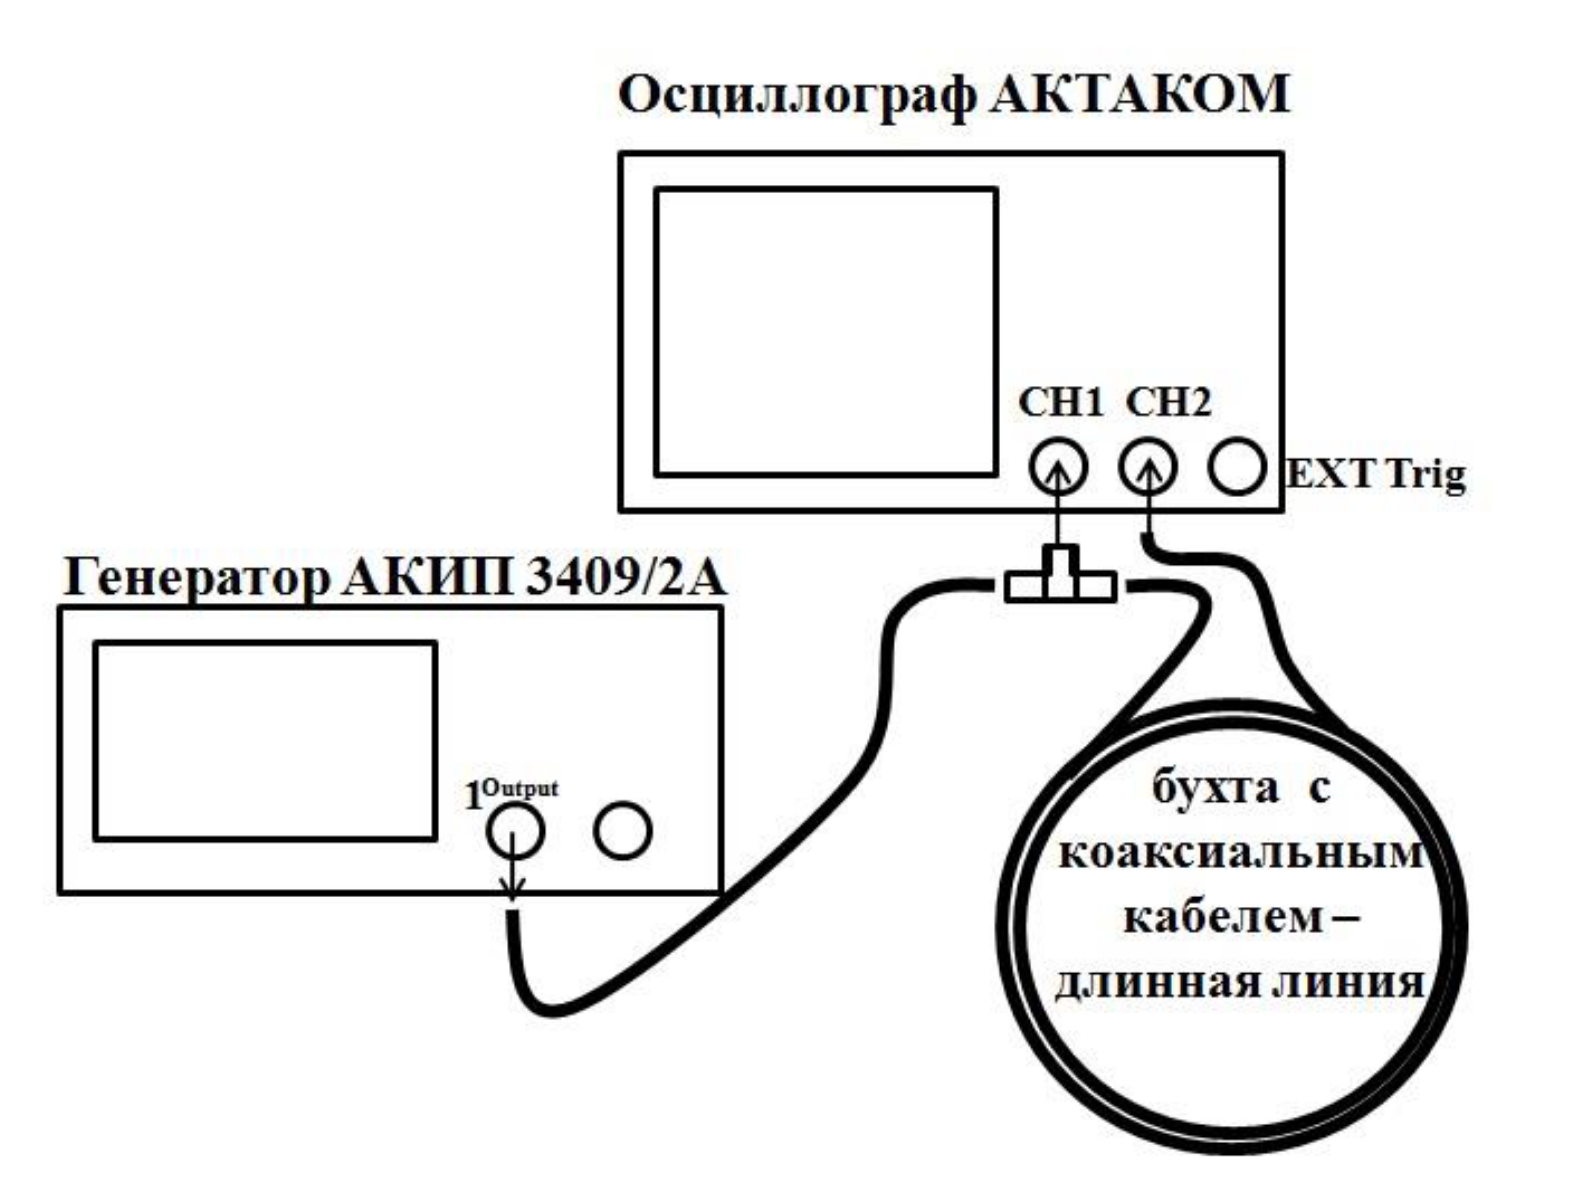
\includegraphics[scale=0.3]{2.png}
    \caption{Схема установки для наблюдения
распространения сигналов вдоль длинной линии.}
    \label{fig:enter-label}
\end{figure}

\begin{table}[H]
    \centering
    \begin{tabular}{|p{2 cm}|p{2 cm}||p{2 cm}|p{2 cm}|}
    \hline
    \multicolumn{2}{|p{4 cm}||}{Нагрузка 50 Ом (согласованная нагрузка)} & \multicolumn{2}{p{2 cm}|}{Нагрузка 1 МОм (линия без нагрузки)} \\
    \hline
    Частота & Сдвиг фаз & Частота & Сдвиг фаз \\
        \hline
    3.88  &  $ 2 \pi$  & 3.76  & $ 2 \pi$\\
\hline
7.84  &  $ 4 \pi$  & 7.93  & $ 4 \pi$\\
\hline
11.79  &  $ 8 \pi$  & 11.89  & $ 8 \pi$\\
\hline
15.73  &  $ 16 \pi$  &  15.86 & $ 16 \pi$ \\
\hline
19.69  &  $ 32 \pi$  & 19.81  & $ 32 \pi$ \\
\hline
23.66  &  $ 64 \pi$  & 23.77  & $64 \pi$ \\
\hline
27.64  &  $ 218 \pi$  & 31.64& $128 \pi$ \\
\hline
    \end{tabular}
    \caption{Резонансные частоты для синусоидального сигнала}
\end{table}


\begin{table}[H]
    \centering
    \begin{tabular}{|p{2 cm}|p{2 cm}||p{2 cm}|p{2 cm}|}
    \hline
    \multicolumn{2}{|p{4 cm}||}{Нагрузка 50 Ом (согласованная нагрузка)} & \multicolumn{2}{p{2 cm}|}{Нагрузка 1 МОм (линия без нагрузки)} \\
    \hline
    Частота & Сдвиг фаз & Частота & Сдвиг фаз \\
        \hline
    3.96  &  $ 2 \pi$  & 3.90  & $ 2 \pi$\\
\hline
7.92  &  $ 4 \pi$  & 7.81  & $ 4 \pi$\\
\hline
11.89  &  $ 8 \pi$  & 11.71  & $ 8 \pi$\\
\hline
15.81  &  $ 16 \pi$  &  15.62 & $ 16 \pi$ \\
\hline
19.75  &  $ 32 \pi$  & 19.52  & $ 32 \pi$ \\
\hline
    \end{tabular}
    \caption{Резонансные частоты для прямоугольного сигнала}
\end{table}


Для синусоидального сигнала и нагрузки 50 Ом построим график зависимости $\nu(n)$
\begin{figure}[H]
    \centering
    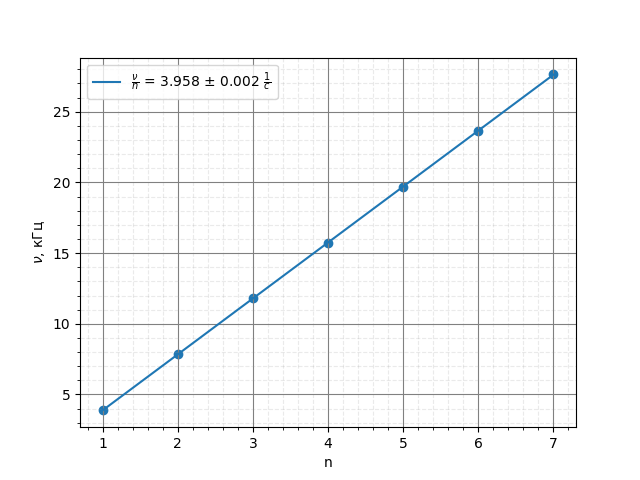
\includegraphics[scale=0.7]{f(n) 50.png}
    \caption{График зависимости $\nu(n)$}
    \label{fig:enter-label}
\end{figure}

Фазовая скорость
\[V_{\text{ф}} = \frac{\nu}{n} \cdot l = 198 \text{ } \frac{\text{cм}}{c}\]

\subsection{АЧХ и ФЧХ}

\begin{table}[H]
    \centering
    \begin{tabular}{|p{2 cm}|p{2 cm}|p{2 cm}|p{2 cm}|}
    \hline
       Частота, МГц  &  Амплитуда входного сигнала, В & Амплитуда выходного сигнала, В & Фаза  \\
    \hline
3.88  &  5.4  &  4.84  & $2\pi$ \\
\hline
7.84  &  5.44  &  4.6  & $4\pi$ \\
\hline
11.79  &  5.48  &  4.44  & $8\pi$ \\
\hline
15.73  &  5.48  &  4.32  & $16\pi$ \\
\hline
19.69  &  5.48  &  4.0  & $32\pi$ \\
\hline
23.66  &  5.4  &  4.08  & $64\pi$ \\
\hline
27.64  &  5.4  &  3.76  & $128\pi$ \\
\hline
31.59  &  5.34  &  3.7  & $256\pi$ \\
\hline
35.55  &  5.33  &  3.63  & $512\pi$ \\
\hline
39.5  &  5.25  &  3.29  & $1024\pi$ \\
\hline
    \end{tabular}
    \caption{АЧХ и ФЧХ}
    \label{tab:my_label}
\end{table}

\subsection{Определение параметров коаксиального кабеля.}


\begin{equation*}
y_{1}=\frac{L_{x} C_{x}}{c^{2}} x_{1} \tag{30}
\end{equation*}


где


\begin{gather*}
x_{1}=\omega^{2},  \tag{31}\\
y_{1}=k(\omega)^{2}-\alpha(\omega)^{2} . \tag{32}
\end{gather*}

\begin{figure}[H]
    \centering
    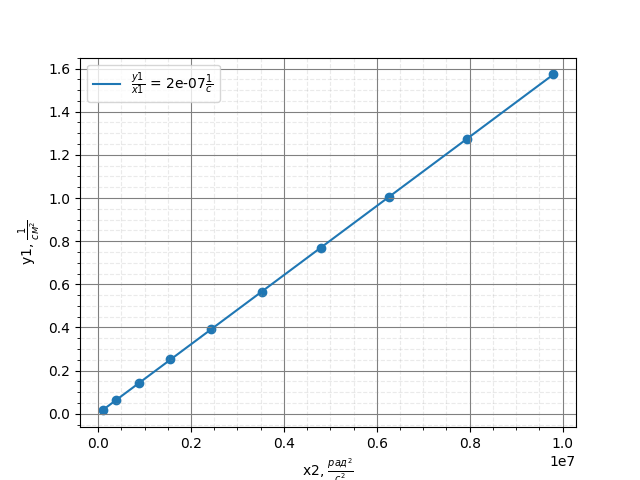
\includegraphics[scale=0.7]{y1(x1).png}
    \caption{$y_1(x_1)$}
    \label{fig:enter-label}
\end{figure}

Из графика 
\[ L_{x} C_{x} = 1.44\]
Тогда
\[L_{x} = 200.2\]
\[C_{x} = 0.0072\]

\[V_{\text{ф}} = \frac{c}{\sqrt{L_{x} C_{x}}} \cdot l = 250 \text{ } \frac{\text{cм}}{c}\]

Магнитная восприимчивость

\[\mu = \frac{L_{x}}{2\log{\frac{r_2}{r_1}}} = 0.93\]
\[\varepsilon = 2C_{x} \log{\frac{r_2}{r_1}} = 1.54\]

\subsection{Определение удельной проводимости проводников.}
\subsubsection{Метод А}


Из (23) и (28) следует:


\begin{equation*}
\alpha(\omega)=\frac{1}{l} \ln \left(\frac{U_{0}}{U_{n}}\right)=R_{x} C_{x} \frac{V_{\phi}}{2} . \tag{33}
\end{equation*}


Если взять удельную проводимость для меди и подставить в известное выражение для характерной толщины скин-слоя:


\begin{equation*}
\delta=\frac{c}{2 \pi \sqrt{v \sigma}}, \tag{34}
\end{equation*}


то окажется, что даже при минимальной частоте $v=1$ МГц эта толщина будет равна около 65 мкм, что примерно в десять раз меньше радиуса центрального проводника (диаметр центральной жилы равен $d=1,37$ мм). При больших частотах характерная толщина скинслоя ещё меньше. Поэтому для упрощения будем предполагать, что весь ток сосредоточен в приповерхностном слое и потери, связанные с джоулевым нагревом описываются следующим выражением:


\begin{equation*}
d N=\left.\sigma E_{0}^{2} \int_{0}^{\infty} e^{-2 \frac{z}{\delta}} d z d x L\right|_{L=\pi d}=\left.\sigma E_{0}^{2} \cdot d x \cdot \pi d \cdot \frac{\delta}{2}\left(-e^{-2 \frac{z}{\delta}}\right)\right|_{0} ^{\infty} \frac{\sigma \cdot \pi d}{d x} \cdot \frac{\delta}{2}(d U)^{2}=\frac{(d U)^{2}}{d R} \tag{35}
\end{equation*}


где


\begin{equation*}
d R=\frac{d x}{\sigma \cdot \pi d} \cdot \frac{2}{\delta} \tag{36}
\end{equation*}


Погонное сопротивление с учётом скин-эффекта можно определить следующим образом:


\begin{equation*}
R_{x}=\frac{d R}{d x}=\frac{2}{\sigma \cdot \pi d \cdot \delta} . \tag{37}
\end{equation*}


Или, с учётом выражения для характерной толщины скин-слоя (34), имеем:


\begin{equation*}
R_{x}=\frac{4 \sqrt{v}}{\sqrt{\sigma} \cdot c \cdot d} \tag{38}
\end{equation*}


Таким образом, подставляя (38) в (33) приходим к зависимости:


\begin{equation*}
\alpha(\omega)=\frac{1}{l} \ln \left(\frac{U_{0}}{U_{u}}\right)=\frac{4}{\sqrt{\sigma} \cdot d} C_{x} \frac{V_{\phi}}{c} \sqrt{v} . \tag{39}
\end{equation*}


Это выражение можно переписать в следующем виде:


\begin{equation*}
y_{2}=\frac{4}{\sqrt{\sigma} \cdot d} C_{x} \frac{V_{\phi}}{c} x_{2} \tag{40}
\end{equation*}


где


\begin{align*}
& x_{2}=\sqrt{v}  \tag{41}\\
& y_{2}=\alpha(\omega) \tag{42}
\end{align*}


\begin{figure}[H]
    \centering
    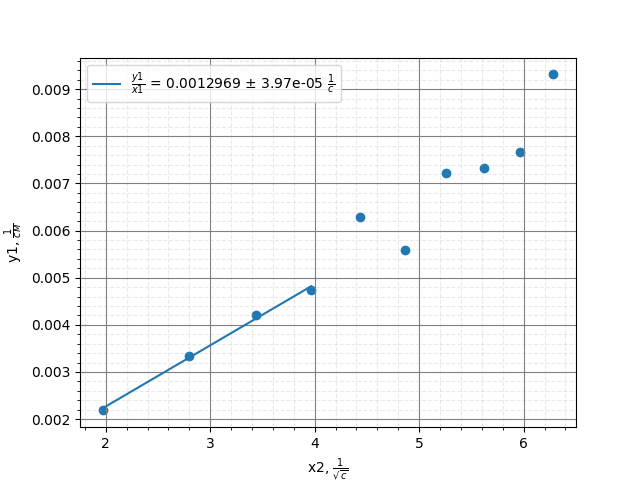
\includegraphics[scale=0.7]{y2(x2).png}
    \caption{$y_2(x_2)$}
    \label{fig:enter-label}
\end{figure}

Отсюда

\begin{equation*}
\sigma=\left(\frac{2 C_{x} V_{\phi}}{c \cdot d \cdot\left(\Delta y_{2} / \Delta x_{2}\right)}\right)^{2} \tag{43}
\end{equation*}

\[\sigma = 4.6\cdot 10^{-18}\]


\subsubsection{Метод Б.}

Подставив выражение для $\gamma$ из (14) во второе уравнение системы (22) и сокращая на квадрат скорости $V_{\phi}^{2}$ легко прийти к выражению:


\begin{equation*}
2 \alpha k=\omega R_{x} C_{x} . \tag{44}
\end{equation*}


Зная амплитуду колебаний и сдвиг фазы в конце длинной линии относительно входного сигнала экспериментально можно определить как $\alpha(\omega)$, так и $k(\omega)$ (см., например, выражения (28) и (29)). Таким образом, выражение (44) можно представить в следующем виде:


\begin{equation*}
y_{3}=\frac{4 \pi \cdot C_{x}}{\sqrt{\sigma} \cdot d \cdot c} x_{3} \tag{45}
\end{equation*}


где


\begin{align*}
& x_{3}=v^{3 / 2},  \tag{46}\\
& y_{3}=\alpha(\omega) \cdot k(\omega)=\frac{1}{l} \ln \left(\frac{U_{0}}{U_{H}}\right) \cdot \frac{\Delta \varphi}{l} . \tag{47}
\end{align*}

\begin{figure}[H]
    \centering
    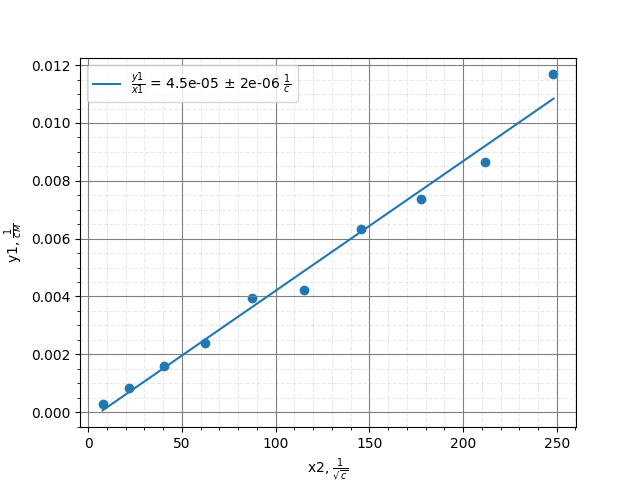
\includegraphics[scale=0.7]{y3(x3).png}
    \caption{Caption}
    \label{fig:enter-label}
\end{figure}




\begin{equation*}
\sigma=\left(\frac{4 \pi \cdot C_{x}}{d \cdot c\left(\Delta y_{3} / \Delta x_{3}\right)}\right)^{2} \tag{48}
\end{equation*}
\[\sigma = 2.4 \cdot 10^{-18}\]



\subsection{Длинная линия. Модель.}
\begin{figure}[H]
    \centering
    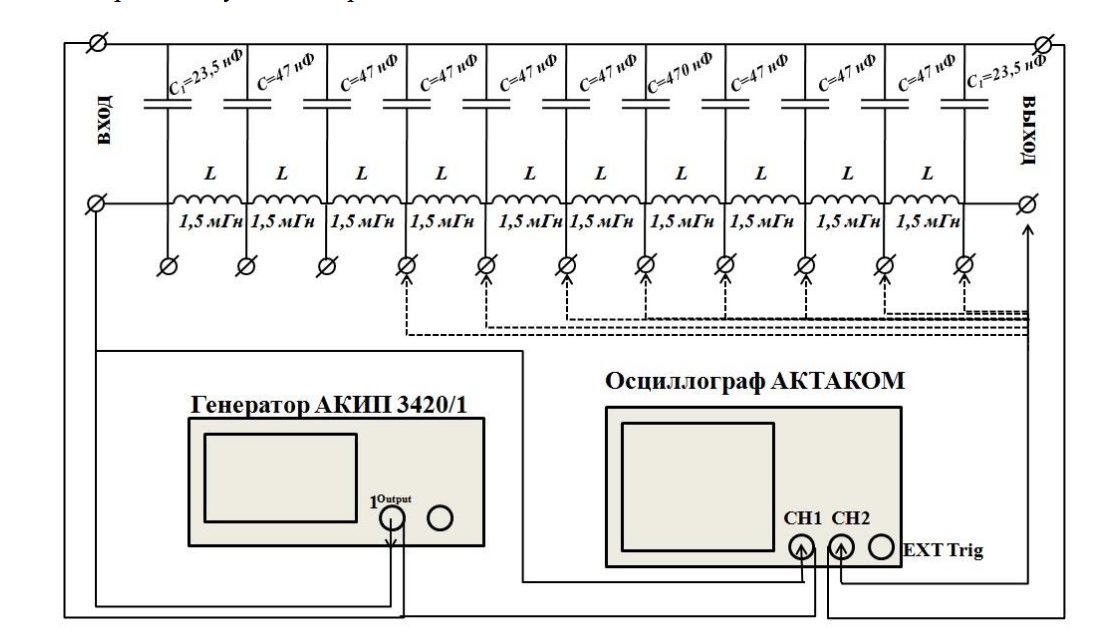
\includegraphics[scale=0.6]{3.png}
    \caption{Модель длинной линии}
    \label{fig:enter-label}
\end{figure}

\begin{equation*}
v_{0}=\frac{1}{\pi \sqrt{L C}} = 38 \text{ кГц} \tag{*}
\end{equation*}


\begin{equation*}
R_{0}=\sqrt{\frac{L}{C}} = 178 \text{ Ом} \tag{**}
\end{equation*}
\begin{table}[H]
    \centering
    \begin{tabular}{|p{2 cm}|p{2 cm}|}
    \hline
    Частота, кГц & Сдвиг фазы, рад \\
    \hline
         1.0  &  0.13 \\
\hline
5.75  &  0.35 \\
\hline
10.5  &  0.66 \\
\hline
15.25  &  0.69 \\
\hline
20.0  &  1.51 \\
\hline
29.5  &  2.3 \\
\hline
34.25  &  2.45 \\
\hline 
    \end{tabular}
    \caption{Сдвиг фазы между двумя соседними ячейками при разных частотах}
    \label{tab:my_label}
\end{table}

\textbf{Наблюдение резонансов}

\begin{table}[H]
    \centering
    \begin{tabular}{|p{2 cm}|p{2 cm}|p{2 cm}|p{2 cm}|p{2 cm}|p{2 cm}|}
    \hline
    \multicolumn{6}{|p{12 cm}|}{R = 0} \\
    \hline
    \multicolumn{2}{|p{4 cm}}{$\nu_{\text{рез}} = 3.25$ кГц}  & \multicolumn{2}{|p{4 cm}}{$\nu_{\text{рез}} = 13.68$ кГц} & \multicolumn{2}{|p{4 cm}|}{$\nu_{\text{рез}} = 23.28$ кГц}  \\
    \hline
    Номер & Амплитуда & Номер & Амплитуда & Номер & Амплитуда \\
    \hline
    1 & 0.24 & 1 & 0.88 & 1 & 1.46  \\
    \hline
    2 & 0.74   & 2 & 2.2 & 2  & 1.94  \\
    \hline
    3 & 1.16   & 3 & 2.24 & 3 & 0.82  \\
    \hline
    4 & 1.6    & 4 & 0.88 & 4 & 2.22  \\
    \hline
    5 & 1.92   & 5 & 0.88 & 5 & 0.72  \\
    \hline
    6 & 2.2    & 6 & 0.88 & 6 & 2.28  \\
    \hline
    7 & 2.4    & 7 & 0.88 & 7 & 1.2  \\
    \hline
    8 & 2.5    & 8 & 0.88 & 8 & 2.44  \\
    \hline
    9 & 2.56   & 9 & 0.88 & 9 & 1.78  \\
    \hline
    10 & 2.58 & 10 & 0.88 & 10 & 2.8  \\
    \hline
    \hline

    
    \multicolumn{6}{|p{12 cm}|}{$R = \infty$} \\
    \hline
    \multicolumn{2}{|p{4 cm}}{$\nu_{\text{рез}} = 10.5$ кГц}  & \multicolumn{2}{|p{4 cm}}{$\nu_{\text{рез}} = 20.2$ кГц} & \multicolumn{2}{|p{4 cm}|}{$\nu_{\text{рез}} = 28.3$ кГц}  \\
    \hline
    Номер & Амплитуда & Номер & Амплитуда & Номер & Амплитуда \\
    \hline
    1  &  2.08  &  1  &  2.52  &  1  &  0.96  \\
    \hline
    2  &  0.92  &  2  &  3.44  &  2  &  3.88  \\
    \hline
    3  &  0.5  &  3  &  4.28  &  3  &  1.12  \\
    \hline
    4  &  1.82  &  4  &  1.28  &  4  &  3.84  \\
    \hline
    5  &  2.5  &  5  &  4.6  &  5  &  3.2  \\
    \hline
    6  &  2.22  &  6  &  3.28  &  6  &  2.96  \\
    \hline
    7  &  1.34  &  7  &  3.8  &  7  &  5.08  \\
    \hline
    8  &  0.62  &  8  &  4.88  &  8  &  3.76  \\
    \hline
    9  &  1.76  &  9  &  3.04  &  9  &  5.6  \\
    \hline
    10  &  2.46  &  10  &  5.52  &  10  &  7.2  \\
    \hline

    
    \end{tabular}
    \caption{Рзонансные частоты и амплитуды на разных клеммах}
    \label{tab:my_label}
\end{table}

\begin{figure}[H]
    \centering
    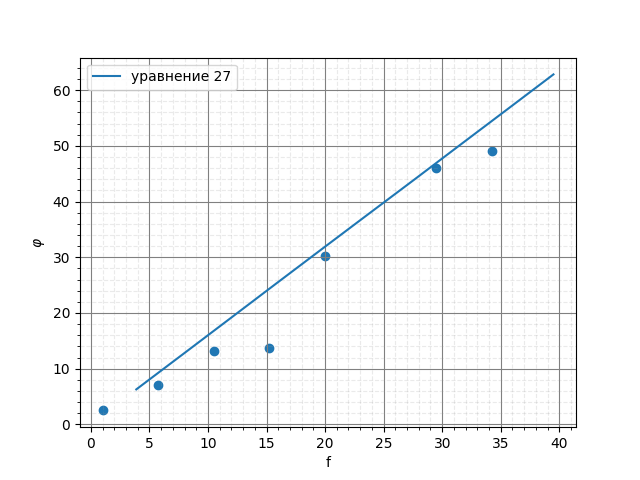
\includegraphics[scale=0.7]{phi(f).png}
    \caption{$\varphi(\nu)$}
\end{figure}



\begin{figure}[H]
    \centering
    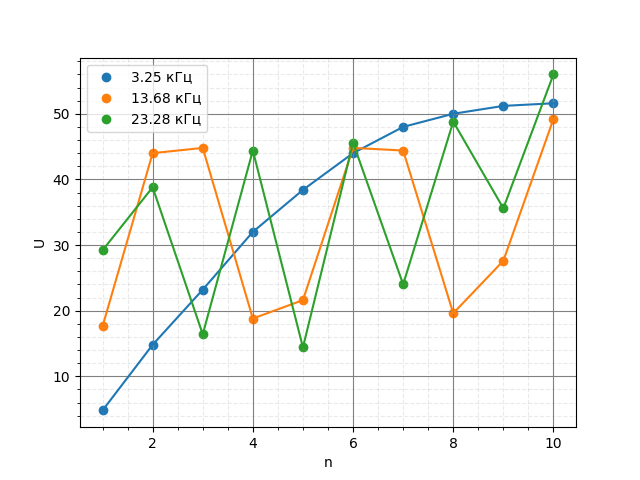
\includegraphics[scale=0.7]{weird1.png}
    \caption{$U(n)$}
\end{figure}








\end{document}


